\documentclass[11pt]{beamer}

\mode<article> {
  \usepackage{beamerbasearticle}
  \usepackage[pdflatex]{hyperref}
}

\usetheme[compress]{Singapore} %Boadilla

% \beamertemplatetransparentcoveredhigh
% \beamertemplatetransparentcovereddynamicmedium

% color themes: albatross crane beetle dove fly seagull wolverine beaver
% \usecolortheme{beaver}
% Outer color themes:whale, seahorse, dolphin
\usecolortheme{whale}
% Inner color themes: lily, orchid,rose
\usecolortheme{orchid}

% available: rectangles circles inmargin rounded
\useinnertheme[shadow]{rounded}
\setbeamertemplate{navigation symbols}{} % no navigation
\useoutertheme{progressbar}

\usefonttheme[onlymath]{serif}
\usepackage[small]{eulervm} % Euler VM for math font
% \usepackage{helvet}

% define colors
\setbeamercolor{uppercol}{fg=white,bg=blue}%
\setbeamercolor{lowercol}{fg=black,bg=gray}%
\xdefinecolor{lavendar}{rgb}{0.8,0.6,1}
\xdefinecolor{olive}{cmyk}{0.64,0,0.95,0.4}
\xdefinecolor{mygreen}{rgb}{0,0.6,0}
\xdefinecolor{mygray}{rgb}{0.5,0.5,0.5}
\xdefinecolor{mymauve}{rgb}{0.58,0,0.82}
\xdefinecolor{mycolor}{rgb}{0.08,0.08,0.16}

%% redefine structure/alert color
% \usecolortheme[named=yellow]{structure}
% \setbeamercolor{alerted text}{fg=mygreen}
% \setbeamercolor{block title alerted}{fg=white,bg=violet!40!gray}
% \setbeamercolor{block body alerted}{fg=black!90,bg=white}
% \setbeamercolor{alerted text}{fg=yellow}
% \setbeamercolor{structured text}{fg=green}
% \setbeamercolor{structure}{fg=beamer@blendedblue}
% \colorlet{structure}{yellow!60!black}
% \colorlet{alert}{green!60!black}

\setbeamertemplate{headline}[default]

% \beamertemplateshadingbackground{blue!5}{yellow!10}
% available: transparent,highly dynamic,dynamic, invisible
\setbeamercovered{invisible}

\setbeamercolor{body}{fg=blue!80, bg=black!20}
\setbeamercolor{head}{fg=blue,bg=blue!30}

% \addtobeamertemplate{block begin}{%
% \setlength{\textwidth}{0.9\textwidth}%
% }{}

\beamertemplateballitem

%% --------------------------------------------------------------------------- %
% math (symbols) related
\usepackage{pifont}
\usepackage{mathrsfs}
\usepackage{bbding}
\usepackage{amsmath, amsfonts, amssymb}
% \usepackage{textcomp}
\usepackage{indentfirst}

% \usepackage{pgf,pgfarrows,pgfnodes,pgfautomata,pgfheaps}
% \usepackage{subfigure}
\usepackage{graphicx}
\usepackage{graphviz}
\usepackage{ccaption}
\graphicspath{{figure/}{fig/}{logo/}{logos/}{graph/}{graphs}}
\DeclareGraphicsExtensions{.pdf,.eps,.png,.jpg,.jpeg}

\usepackage{fancybox} %including shadowbox,fbox,Ovalbox,ovalbox,doublebox
\usepackage{multimedia}
\usepackage{listings}
\usepackage{boxedminipage}
\usepackage{multirow, multicol, pdflscape}
\usepackage{array}
\usepackage{ulem,soul}
% \usepackage{enumitem}
\usepackage[lined,boxed,ruled,linesnumbered]{algorithm2e}

\usepackage{times}
% \usepackage[tikz]{bclogo}
\usepackage{tikz}
\usetikzlibrary{shapes, arrows}

% definitions

\makeatletter
\newenvironment{CenteredBox}{
  \begin{Sbox}}{
  \end{Sbox}\centerline{\parbox{\wd\@Sbox}{\TheSbox}}}
\makeatother

\newenvironment<>{varblock}[2][\textwidth]{
  \setlength{\textwidth}{#1}
  \begin{actionenv}#3
    \def\insertblocktitle{#2}
    \par
    \usebeamertemplate{block begin}}
  {\par
    \usebeamertemplate{block end}
  \end{actionenv}}

\makeatletter
\def\beamer@linkspace#1{
  \begin{pgfpicture}{0pt}{-1.5pt}{#1}{5.5pt}
    \pgfsetfillopacity{0}
    \pgftext[x=0pt,y=-1.5pt]{.}
    \pgftext[x=#1,y=5.5pt]{.}
  \end{pgfpicture}}
\makeatother


\AtBeginSection[]{
  \frame<handout:0>{
    \frametitle{Outline}
    \tableofcontents[current,currentsubsection,shaded]
  }
  \addtocounter{framenumber}{-1}
}

\hypersetup{pdfpagemode={FullScreen}}
\hypersetup{pdfstartview={FitH}}
\setbeamertemplate{itemize/enumerate body begin}{\small}
\setbeamertemplate{itemize/enumerate subbody begin}{\footnotesize}

\lstset{
  backgroundcolor=\color{white!90!yellow},   % choose the background color
  basicstyle=\color{black}\ttfamily\tiny,    % the size of the fonts that are used for the code
  breakatwhitespace=false,                   % sets if automatic breaks should only happen at whitespace
  breaklines=true,                           % sets automatic line breaking
  captionpos=b,                              % sets the caption-position to bottom
  commentstyle=\color{mygray}\itshape,       % comment style
  deletekeywords={...},                      % if you want to delete keywords from the given language
  escapeinside={\%*}{*)},                    % if you want to add LaTeX within your code
  extendedchars=true,                        % lets you use non-ASCII characters; for 8-bits encodings only, does not work with UTF-8
  frame=single,                              % adds a frame around the code
  keepspaces=true,                           % keeps spaces in text, useful for keeping indentation of code (possibly needs columns=flexible)
  keywordstyle=\color{blue!70},              % keyword style
  identifierstyle=\texttt,
  % language=C,                               % the language of the code
  morekeywords={*,...},                      % if you want to add more keywords to the set
  numbers=left,                              % where to put the line-numbers; possible values are (none, left, right)
  numbersep=5pt,                             % how far the line-numbers are from the code
  numberstyle=\tiny\color{mygray},           % the style that is used for the line-numbers
  rulecolor=\color{black},                   % if not set, the frame-color may be changed on line-breaks within not-black text
  showspaces=false,                          % show spaces everywhere adding particular underscores; it overrides 'showstringspaces'
  showstringspaces=false,                    % underline spaces within strings only
  showtabs=false,                            % show tabs within strings adding particular underscores
  stepnumber=1,                              % the step between two line-numbers. If it's 1, each line will be numbered
  stringstyle=\color{mymauve},               % string literal style
  tabsize=2,                                 % sets default tabsize to 2 spaces
  upquote=true,
  title=\lstname                             % show the filename of files included with \lstinputlisting; also try caption instead of title
}

% for title page
% \setbeamerfont{title}{shape=\slshape,family=\ttfamily,series=\bfseries}
\title{Search Strategies in Symbolic Execution}
\author{Presented by CHEN Hongxu}
\date{July 8, 2014}

%% --------------------------------------------------------------------------- %

\begin{document}

\frame{\titlepage}

\section{Fundamentals}

\begin{frame}
  \frametitle{Symbolic Execution}
  \begin{itemize}
  \item Execute programs with \alert{symbol values} rather than concrete inputs
  \item Keep path conditons and let solver to decide the satisfiability
  \item[\ding{51}] Explore execution space systematically
  \item[\ding{51}] Generate tests with higher coverage
  \item[\ding{55}] Suffer from \uline{\structure{path explosion}}
  \end{itemize}
  \begin{center}
    \shadowbox{Proper path search strategies}
  \end{center}
\end{frame}

\section{Path Selection Strategies}

\begin{frame}
  \frametitle{Concolic Execution}
  \begin{itemize}
  \item Use \alert{concrete} execution to produce a \structure{trace} of a program execution. \alert{Forward symbolic} execution then follows \structure{the same path}
  \item Generate other conditions by negating the conditons in later branch conditions
  \item[\ding{51}] Faster than traditional symbolic execution
  \item[\ding{51}] Bypass some of the difficulties for NON-linear constraints solving or library calls
  \item[\ding{55}] Miss lots of cases during negating the path regarding to
    concrete value
  \item[\ding{43}] Tools: CUTE(FSE2005),  DART(PLDI2005)
  \end{itemize}
\end{frame}

\begin{frame}[containsverbatim]
  \frametitle{Concolic Execution -- An Example}
  \begin{columns}
    \column{.5\textwidth}
\begin{lstlisting}[language=C]
int double(int x) {
  return 2 * x;
}

void test_me(int x, int y) {
  int z = double(x);
  if (z == y) {
    if (x != y + 10) {
      printf("I am fine here");
    } else {
      printf("I should not reach here");
      abort();
    }
}
\end{lstlisting}
\begin{lstlisting}[language=C, numbers=none]
int main(void){
    int t1 = randomInt();
    int t2 = randomInt();
    test_me(t1,t2);
    return 0;
}
\end{lstlisting}
    \column{.4\textwidth}
    \begin{block}{}
      \begin{enumerate}
      \item $t_1:=36, t_2:=-7 \Rightarrow \alert{z=y\Big{|}_{\#7}}$
      \item $t_1:=1, t_2=:2 \Rightarrow z\neq y\Big{|}_{\#7} \wedge \alert{x\neq y+10\Big{|}_{\#8}} $
      \item $t_1:=-10, t_2:=-20 \Rightarrow z\neq y\Big{|}_{\#7} \wedge \uline{x=y+10\Big{|}_{\#8}}$
      \end{enumerate}
    \end{block}
  \end{columns}

\end{frame}

\begin{frame}
  \frametitle{Depth-First-Search(DFS)}
  \begin{itemize}
  \item Select the LATEST execution state
  \item[\ding{51}] Little overhead in selecting a state
  \item[\ding{55}] lower statement/branch coverage
  \item[\ding{55}] get stuck when encountering loops
  \item[\ding{43}] KLEE(OSDI2008)
  \end{itemize}
\end{frame}

\begin{frame}
  \frametitle{Random State Search(RSS)}
  \begin{itemize}
  \item Randomly select a pending state to explore
  \item[\ding{51}] explore programs uniformly
  \item[\ding{51}] avoid tight loops with a symbolic condition creating new states
  \item[\ding{55}] may generate redundant test cases
  \item[\ding{43}] KLEE(OSDI2008)
  \end{itemize}
\end{frame}

\begin{frame}
  \frametitle{Random Path Selection(RPS)}
  \begin{itemize}
  \item Use a binary execution tree to record information on explored program parts
    \begin{itemize}
    \item leaves: current states
    \item internal nodes: forks
    \end{itemize}
  \item Select state by traversing tree from root and randomly pick a
    direction when encountering a branch until reaching a leaf
  \item[\ding{51}] favor states high in the branch tree
  \item[\ding{51}] avoid starvation when part of the program is rapidly creating new states
  \item[\ding{51}] avoid fork bombing affecting DFS
  \item[\ding{55}] may still generate similar test cases
  \item[\ding{43}] KLEE(OSDI2008)
  \end{itemize}
\end{frame}

\begin{frame}
  \frametitle{Coverage-Optimized Search(COS)}
  \begin{itemize}
  \item Use heuristics to compute which state has better chance to cover new code
  \item Calculate a weight and select states w.r.t. the weight
  \item Various weights(not general)
    \begin{description}
    \item [nurs:covnew]  Non Uniform Random Search (NURS) with Coverage-New heuristic
    \item [nurs:md2u  ]  NURS with Min-Dist-to-Uncovered heuristic
    \item [nurs:depth ]  NURS with $2^{depth}$ heuristic
    \item [nurs:icnt  ]  NURS with Instr-Count heuristic
    \item [nurs:cpicnt]  NURS with CallPath-Instr-Count heuristic
    \item [nurs:qc    ]  NURS with Query-Cost heuristic
    \end{description}
  \item[\ding{51}] Should gain the highest coverage
  \item[\ding{55}] May not work for every program
  \item[\ding{43}] KLEE(OSDI2008)
  \end{itemize}
\end{frame}


\begin{frame}
  \frametitle{Subpath-Guided Search(SGS)}
  \begin{itemize}
  \item Profiling based Symbolic Execution using length-n spectra
  \item[\ding{51}] Priorize ``less traveled'' paths to improve coverage
  \item[\ding{43}] Steering Symbolic Execution to Less Traveled Paths (OOPSLA2013)
  \item Approximate full paths information\linebreak\linebreak
    Full path:
    \begin{equation}
      \pi=\langle s_0, s_1, \ldots s_k \rangle\label{eq:1}
    \end{equation}
    $length-n$ subpath:
    \begin{equation}
      \pi_{i,n}=\langle s_i+1, s_i+2, \ldots s_n \rangle\label{eq:2}
    \end{equation}
    \begin{itemize}
    \item $n=1$ $\Rightarrow$ branch coverage
    \item $n=\infty$ $\Rightarrow$ path coverage
    \end{itemize}
  \end{itemize}
\end{frame}

\begin{frame}
  \frametitle{SGS -- An Example}
  \begin{center}
    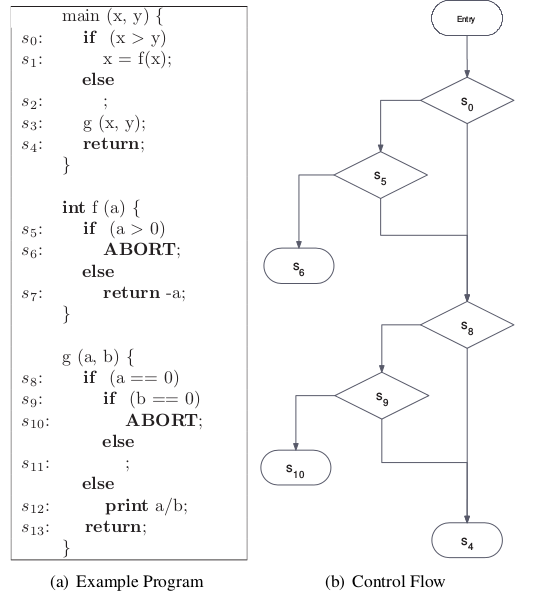
\includegraphics[totalheight=0.8\textheight]{example.png}
  \end{center}
\end{frame}

\begin{frame}
  \frametitle{SGS Algorithm (Part 1)}
  \begin{columns}
    \column{.45\textwidth}
    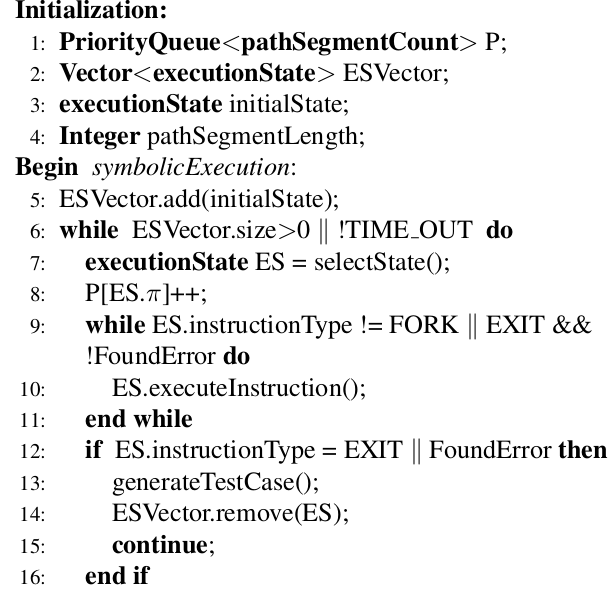
\includegraphics[totalheight=0.6\textheight]{SGS_1_1.png}
    \column{.45\textwidth}
    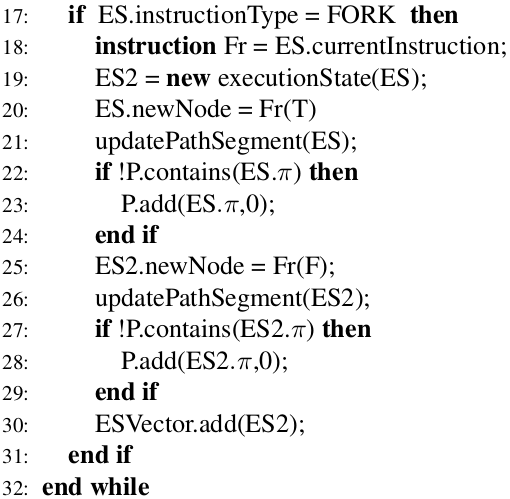
\includegraphics[totalheight=0.6\textheight]{SGS_1_2.png}
  \end{columns}
\end{frame}

\begin{frame}
  \frametitle{SGS Algorithm (Part 2)}
  \begin{center}
    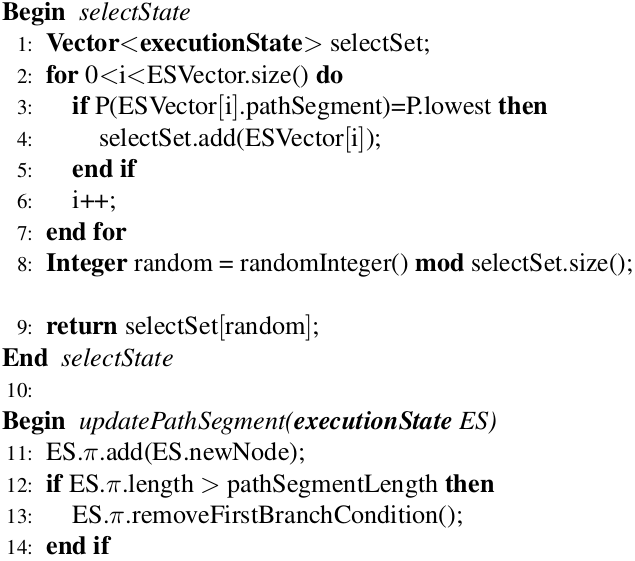
\includegraphics[totalheight=0.8\textheight]{SGS_2.png}
  \end{center}
\end{frame}

\begin{frame}
  \frametitle{Length-1 Subpath}
  \begin{center}
    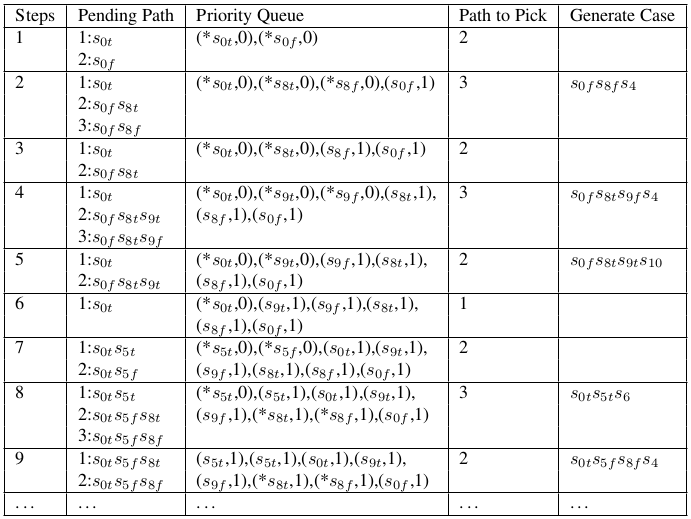
\includegraphics[totalheight=0.8\textheight]{Len1.png}
  \end{center}
\end{frame}

% \begin{frame}
%   \frametitle{Length-2 Subpath}
%   \begin{center}
%     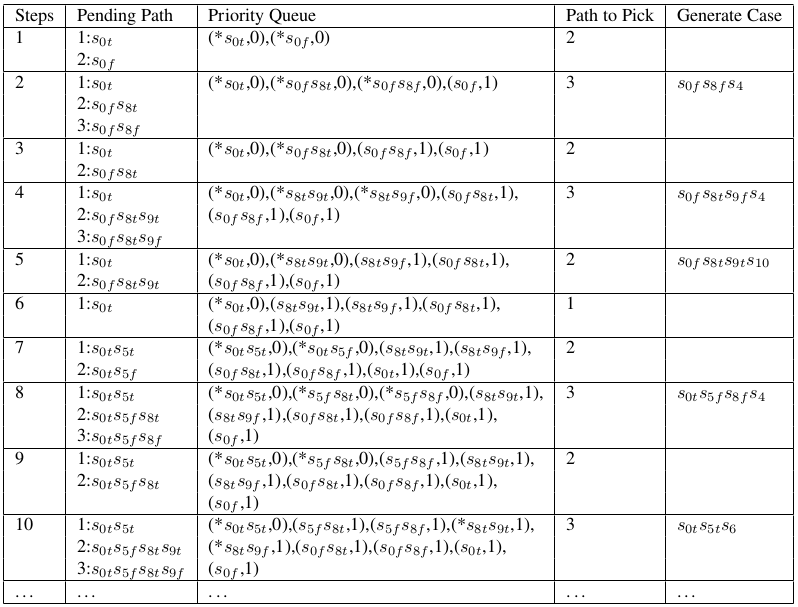
\includegraphics[totalheight=0.8\textheight]{Len2.png}
%   \end{center}
% \end{frame}

\begin{frame}
  \frametitle{Redundant State Detection}
  \begin{itemize}
  \item \textbf{Insight} Prune states that must execute identically to a previously explored state
  \item \textbf{Goal}: high-coverage test case generation
  \item \textbf{Challenge}: how to detect redundant w/o executing it $\Leftarrow$ We do not know in advance what lines a state will cover
  \item \textbf{Approach}: compare state to previously executed states to see
    if it definitely does not cover a new line of code
  \item[\ding{43}] Redundant State Detection for Dynamic Symbolic Execution(atc2013)
  \end{itemize}
\end{frame}

\begin{frame}
  \frametitle{Redundant State Detection -- An Example}
  \begin{center}
    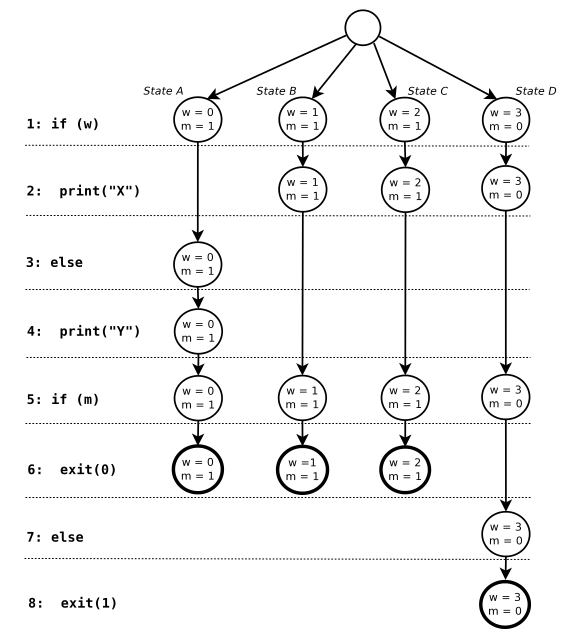
\includegraphics[height=.9\textheight]{detector_eg.png}
  \end{center}
\end{frame}

\begin{frame}
  \frametitle{Redundant State Dection Algorithm}
  \begin{center}
    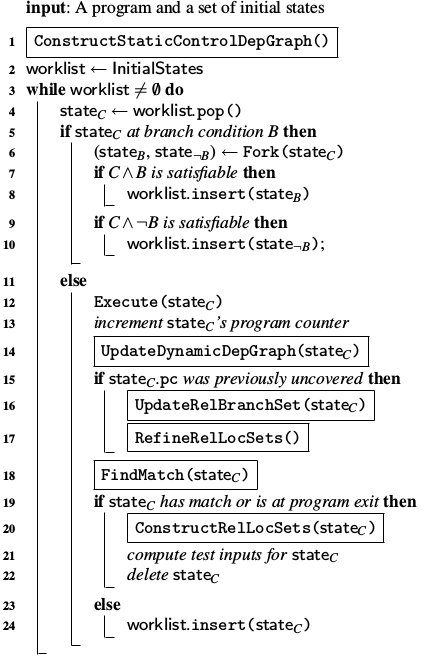
\includegraphics[height=.9\textheight]{detector.png}
  \end{center}
\end{frame}

\begin{frame}
  \frametitle{Rule-Directed Symbolic Execution}
  \begin{itemize}
  \item \textbf{Insight:} For a checked rule, only a portion of \alert{paths} are relevant
    \begin{itemize}
    \item[-] the rest(majority) \alert{paths} do not need to be verified
    \end{itemize}
  \item Modeled Rules:
    \begin{enumerate}[i]
    \item Assertion
    \item Memory Leak
    \item File Open/Close pairs
    \item File Read/Write when opened
    \item Data Loss(e.g. atomic \uline{\textsl{rename}})
    \end{enumerate}
  \item Woodpecker(ASPLOS2013)
  \end{itemize}
\end{frame}

\begin{frame}
  \frametitle{Rule-Directed Symbolic Execution -- An Example}
  \begin{columns}
    \column{.5\textwidth}
    \begin{center}
      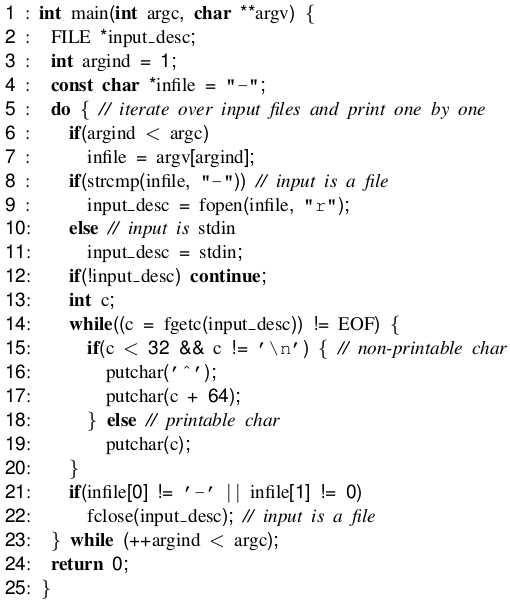
\includegraphics[width=.95\textwidth]{woodpecker_eg.png}
    \end{center}
    \column{.4\textwidth}
    \begin{center}
      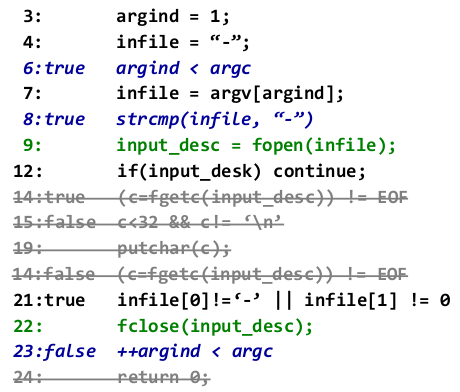
\includegraphics[width=.95\textwidth]{woodpecker_result.png}
    \end{center}
  \end{columns}
\end{frame}

\begin{frame}
  \frametitle{Rule-Directed Symbolic Execution -- Architecture}
  \begin{columns}
    \column{.55\textwidth}
    \begin{center}
      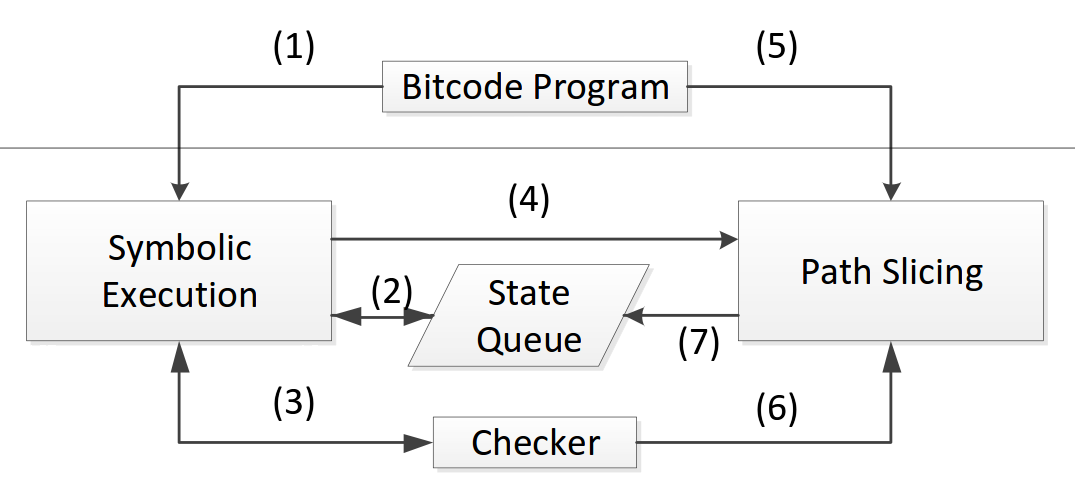
\includegraphics[width=.9\textwidth]{woodpecker.png}
    \end{center}
    \column{.45\textwidth}
    \begin{enumerate}[(1)]
      \tiny{
      \item Given a \structure{bitcode program}, invoke KLEE to interpret instructions
      \item If executing an instruction(e.g., BranchInst) on a state leads to \uline{\textsc{new}} states, adds to the \structure{state queue} for future exploration
      \item Pass executed instruction and its operands to the \structure{checker} for errors
      \item If the instruction executed is at the \uline{end} of a path, apply \ovalbox{\structure{\textsc{path slicing}}} to compute \uline{redundant} branches(w.r.t \uline{event sequence})
      \item As part of the computation to determine if a branch is redundant, \uline{statically} visit off-the-path instructions a branch may reach.
      \item For each instruction visited, \structure{checker} to determine whether the instruction may be an \uline{event}.
      \item Given the redundant branches, search a branch tree to find the corresponding states \uline{forked} from the branches, and \uline{removes} the states from the queue.
      }
    \end{enumerate}
  \end{columns}
\end{frame}

\begin{frame}[containsverbatim]
  \frametitle{Path Slice}
  \begin{columns}
    \column{.4\textwidth}
    A \uline{path slice}{(PLDI2005)} is a subsequence $\pi^\prime$  of a path $\pi$, which is:
    \begin{itemize}
    \item \textbf{Sound:} $\forall s\in S$, $s$ can execute $\pi$
      $\Rightarrow$ $s$ can execute $\pi^\prime$
    \item \textbf{Complete:}
      \begin{enumerate}
      \item There exists a path $\pi^{\prime\prime}$ from $pc_{0}$ to $pc_\varepsilon$ s.t. s
        can execute $\pi^{\prime\prime}$
      \item s cannot reach $pc_{out}$
      \end{enumerate}
    \end{itemize}
    \column{.5\textwidth}
\begin{lstlisting}[language=C]
void MyExample(int a) {
  int counter = 0;
  int *myPointer = NULL ;
  int increment = anyFunction();
  while (counter < a)
  counter += increment;
  if (counter == 0)
  counter = myPointer[0];
  // ERROR Location
}
\end{lstlisting}
  \end{columns}
\end{frame}


\end{document}

% LocalWords:  mycolor mymauve mygray LocalWords png Subpath
